\subsection{Pseudospectral Methods\label{sec:app3:ps}}

This section outlines how to determine the nodes, differentiation matrix, and quadrature weights for use in pseudospectral methods.

\subsubsection{Legendre Pseudospectral Method with LGL Nodes\label{sec:app3:sLGL}}

Let $L_N(\tau)$ denote the Legendre polynomial of order $N$, which may be generated from:
\begin{align}
L_N(\tau) = \frac{1}{2^N N!} \frac{d^N}{d\tau^N}\left(\tau^2 - 1 \right)^N
\end{align}

\noindent The Lagrange-Gauss-Lobatto (LGL) nodes are defined as:
\begin{align}
\tau_k = \begin{cases} -1 & \text{if } k = 0 \\
k\text{th root of } \dot{L}_{N_t}(\tau) & \text{if } k = \{1,2,\dots,N_t-1\} \\
 1 & \text{if } k = N_t 
\end{cases}
\end{align}

\noindent where $\dot{L}_{N} = \frac{dL_{N}}{d\tau}$. We note that the nodes are always between $\left[-1,1\right]$ and contain both endpoints (Ref.~\cite{github-basic-multiple-interval-pseudospectral} codes from Ref.~\cite{Shen2011a}).

We define the basis polynomials needed in Eqn.~(\ref{eq:ch5:basis}) for the Legendre-based method as Lagrange basis polynomials:
\begin{equation}
\phi_k(\tau) = \prod_{i=0,i\neq k}^{N_t} \frac{\tau - \tau_i}{\tau_k - \tau_i} \label{eq:lagrangepoly}
\end{equation}

\noindent With LGL nodes, $\phi_k(\tau)$ can be written in the following alternative form \cite{Becerra2010b}:
\begin{align}
\phi_k(\tau) &= \frac{1}{N_t\left(N_t + 1\right) L_{N_t}(\tau_k)} \frac{(\tau^2 - 1) \ensuremath{\dot{L}}_{N_t}(\tau)}{\tau-\tau_k}
\end{align}

The differentiation matrix needed in Eqn.~(\ref{eq:ch5:ps:state:approx}) for the Legendre-based method is:
\begin{align}
D_{ki} &= \begin{cases}
\frac{L_{N_t}(\tau_k)}{L_{N_t}(\tau_i)} \frac{1}{\tau_k - \tau_i} & \text{if } k \neq i \\
{N_t}({N_t}+1)/4 & \text{if } k = i = 0 \\
-{N_t}({N_t}+1)/4 & \text{if } k = i = {N_t} \\
0 & \text{otherwise}
\end{cases}
\end{align}

\noindent Further numerical enhancements can be made to improve stability in the presence of rounding errors (expression from Ref.~\cite{Becerra2010b}, Ref.~\cite{github-basic-multiple-interval-pseudospectral} codes from Ref.~\cite{Shen2011a}).

The quadrature weights ${w}_k$ needed in Eqn.~(\ref{eq:ch5:gaussian}) for the Legendre-based method are:
\begin{align}
{w}_k = \frac{2}{N_t(N_t+1)} \frac{1}{\left(L_{N_t}(\tau_k)\right)^2}, \qquad k = \{0,1,\dots,N_t\}
\end{align}

\noindent These are Gaussian quadrature weights that are exactly accurate for polynomials of degree up to degree $2N_t - 1$ (expression from Ref.~\cite{Fahroo2008a}, Ref.~\cite{github-basic-multiple-interval-pseudospectral} codes from Ref.~\cite{Shen2011a}).

\subsubsection{Chebyshev Pseudospectral Method with CGL Nodes \label{sec:app3:sCGL}}

Let $T_N(\tau)$ denote the Chebyshev polynomial of order $N$, which may be generated from:
\begin{align}
T_{N} = \cos\left( N \cos^{-1}\left(\tau\right)\right)
\end{align}

\noindent The Chebyshev-Gauss-Lobatto (CGL) nodes are defined as the roots of $\dot{T}_{N_t} = \frac{d{T}_{N_t}}{d\tau}$ and the additional endpoints. All CGL nodes can be computed conveniently by:
\begin{align}
\tau_k = -\cos\left(\frac{\pi k}{N_t} \right) \qquad k = \{0,1,\dots,N_t \}
\end{align}

\noindent We note that the nodes are always between $[-1,1]$ and contain both endpoints.

We define the basis polynomials needed in Eqn.~(\ref{eq:ch5:basis}) for the Chebyshev-based method as Lagrange basis polynomials previously defined in Eqn.~(\ref{eq:lagrangepoly}). With CGL nodes, $\phi_k(\tau)$ can be written in the following alternative form \cite{Fahroo2002a}:
\begin{align}
\phi_k(\tau) = \frac{(-1)^{k+1}}{N_t^2 a_k} \frac{(1-\tau^2)\ensuremath{\protect\dot{T}}_{N_t}(\tau)}{\tau - \tau_k} \quad \text{where: } a_k = \begin{cases} 2 & \text{if } k = \{0,N_t\} \\ 1& \text{otherwise}\end{cases}
\end{align}

The differentiation matrix needed in Eqn.~(\ref{eq:ch5:ps:state:approx}) for the Chebyshev-based method is:
\begin{align}
D_{ki} &= \begin{cases}
\frac{a_k}{a_i} \frac{(-1)^{k+i}}{(\tau_k-\tau_i)} & \text{if } k \neq i \\
-\frac{\tau_k}{2(1-\tau_k^2)} & \text{if } 1 \leq k = i \leq {N_t} - 1 \\
\frac{2N_t^2 + 1}{6} & \text{if } k = i = 0 \\
-\frac{2N_t^2 + 1}{6} & \text{if } k = i = {N_t}
\end{cases}
\end{align}

\noindent Further numerical enhancements can be made to improve stability in the presence of rounding errors (expression from Ref.~\cite{Fahroo2002a}, Ref.~\cite{github-basic-multiple-interval-pseudospectral} codes from \cite[p.~54]{Trefethen2000a}).

The quadrature weights ${w}_k$ needed in Eqn.~(\ref{eq:ch5:gaussian}) for the Chebyshev-based method are:
\begin{gather}
{w}_k =  \frac{c_k}{N_t}\left(1 - \sum_{j=1}^{\lfloor N_t/2\rfloor} \frac{b_j}{4j^2 - 1} \cos\left(2j\tau_k \right) \right) \\
 \text{where: } {b_j} = \begin{cases} 1 & \text{if } j = N_t/2 \\ 2& \text{if } j < N_t/2 \end{cases},  \qquad {c}_k = \begin{cases} 1 & \text{if } k = \{0,N_t\}  \\ 2& \text{otherwise} \end{cases} \notag
\end{gather}

\noindent These are Clenshaw-Curtis quadrature weights that are exactly accurate for polynomials of degree up to degree $N_t$ (expression from Ref.~\cite{Waldvogel2006a}, Ref.~\cite{github-basic-multiple-interval-pseudospectral} codes from Ref.~\cite[p.~128]{Trefethen2000a}).


\subsubsection{Visualizations for Specific Pseudospectral Implementations}

This sections contains a number of visualizations devoted to explaining the various aspects of the specific pseudospectral methods outlined in Secs.~\ref{sec:app3:sLGL} and \ref{sec:app3:sCGL}. Many of the figures are similar to the ones found in Refs.~\cite{Becerra2010b, Becerra2015a} so please refer to them for further analysis.

\noindent\begin{figure}[!h]
\centering
\begin{subfigure}[b]{0.45\textwidth}
\begin{center}
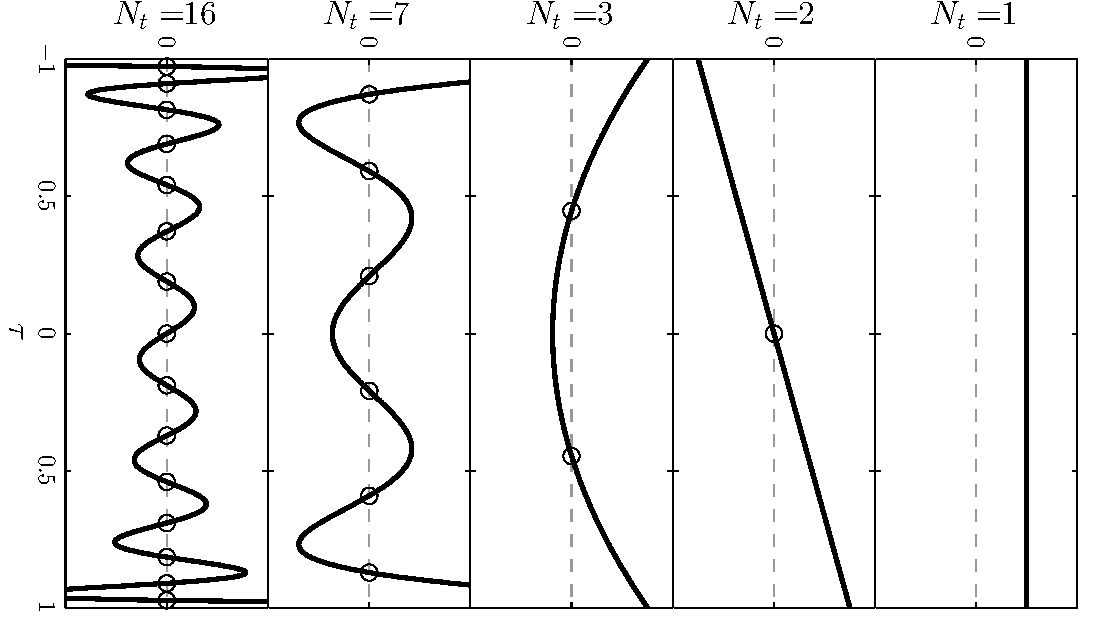
\includegraphics[height=0.25\textheight,angle=90]{../app3/figures/LGLpoly}
\caption{Inner LGL nodes based on $\dot{L}_{N_t}(\tau)$. \label{fig:LGLpoly}}
\end{center}
\end{subfigure}%
\begin{subfigure}[b]{0.45\textwidth}
\begin{center}
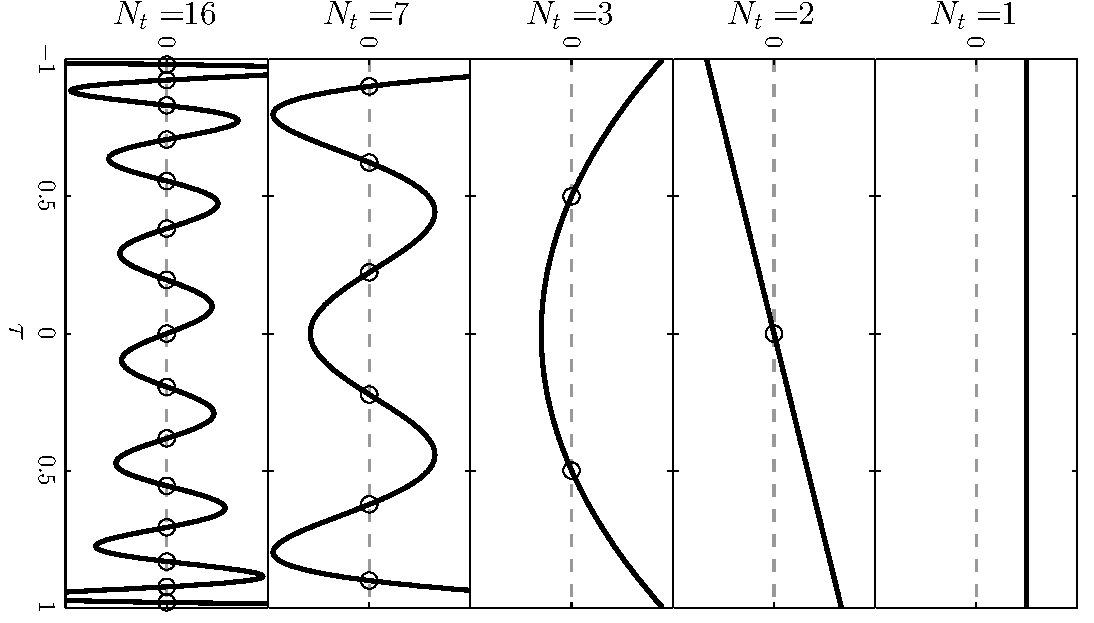
\includegraphics[height=0.25\textheight,angle=90]{../app3/figures/CGLpoly}
\caption{Inner CGL nodes based on $\dot{T}_{N_t}(\tau)$. \label{fig:CGLpoly}}
\end{center}
\end{subfigure}

\caption[LGL and CGL inner node locations from the roots of polynomials]{LGL and CGL inner node locations from the roots of polynomials. \label{fig:node-compare}}
\end{figure}

\begin{figure}
\centering
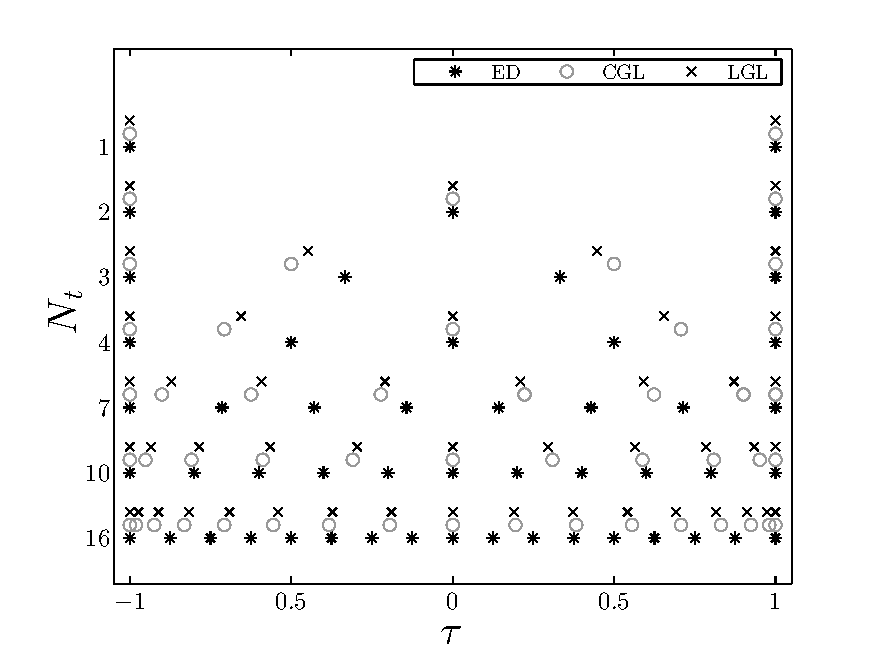
\includegraphics[width=0.6\textwidth]{../app3/figures/nodes}
\caption[ED, CGL, and LGL nodes for various values of $N_t$]{ED, CGL, and LGL nodes for various values of $N_t$. \label{fig:nodes}}
\end{figure}

\begin{figure}
\centering
{\large$f(\tau) = \frac{1}{1 + \tau + 15\tau^2}$}\\
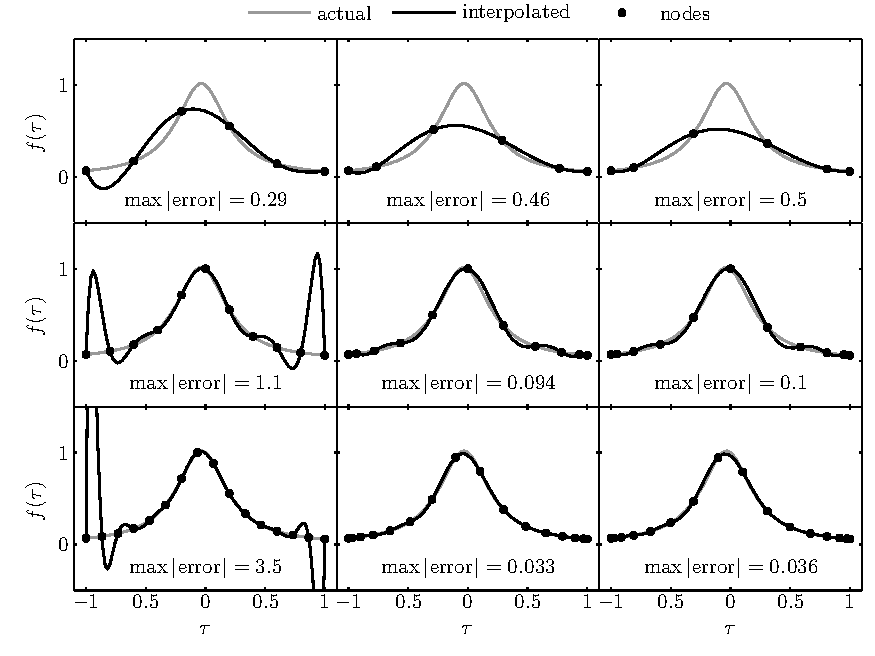
\includegraphics[width=0.8\textwidth]{../app3/figures/approx}
\caption[Lagrange polynomial interpolation with ED, LGL, and CGL
nodes]{Lagrange polynomial interpolation with ED, LGL, and CGL
nodes for various values of $N_t$. \label{fig:approx}}
\end{figure}

\begin{figure}
\centering
\begin{subfigure}[b]{0.6\textwidth}
\centering
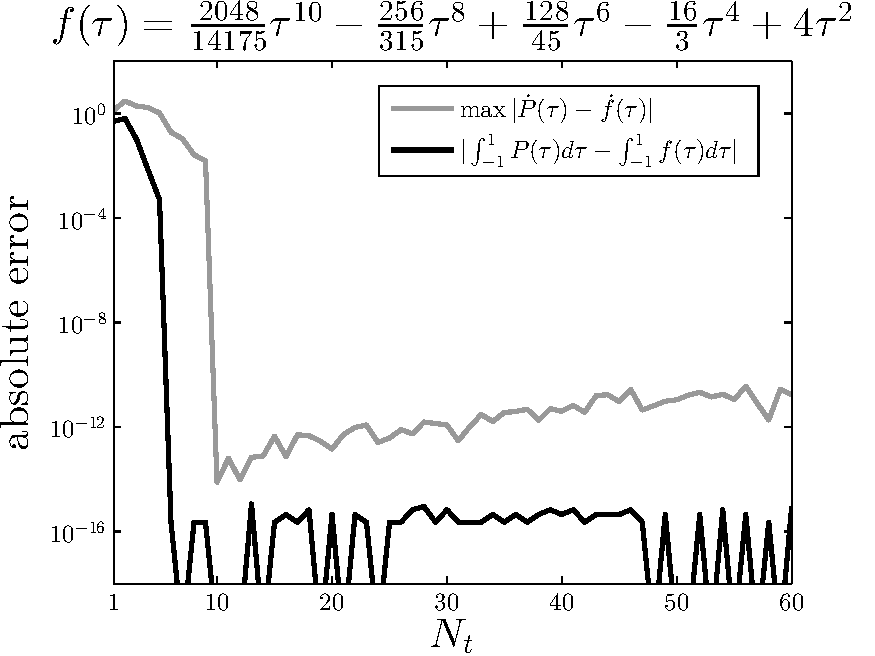
\includegraphics[width=\textwidth]{../app3/figures/integration-1}
\caption{Polynomial example. \label{fig:int-1}}
\end{subfigure}

\begin{subfigure}[b]{0.6\textwidth}
\centering
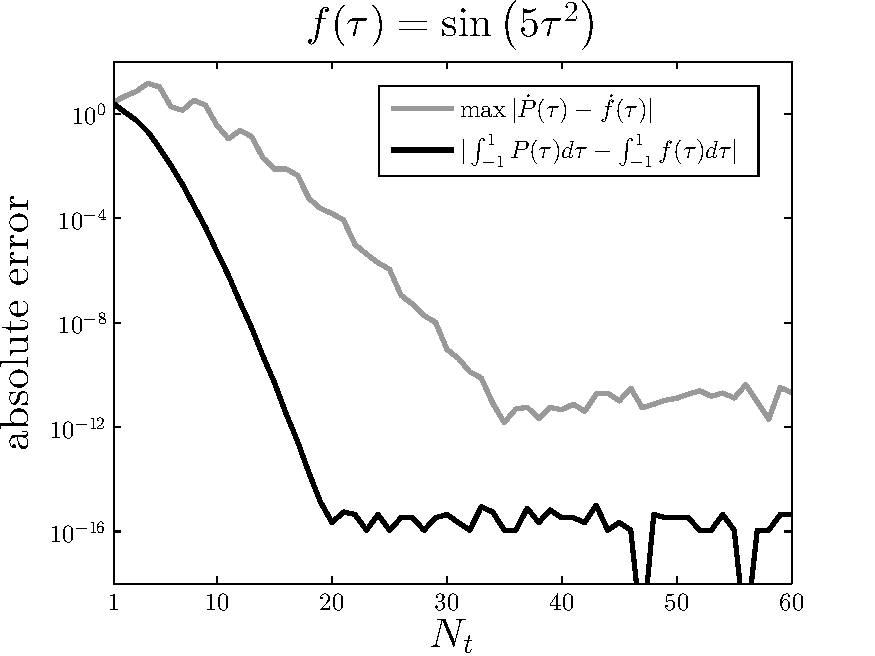
\includegraphics[width=\textwidth]{../app3/figures/integration-2}
\caption{Nonpolynomial example. \label{fig:int-2}}
\end{subfigure}

\caption[Convergence behavior for definite integral and derivative approximations using Lagrange interpolation with LGL nodes]{Convergence behavior for definite integral and derivative approximations using Lagrange interpolation with LGL nodes. \label{fig:int}}
\end{figure}

\begin{figure}
\centering
{\large$f(\tau) = \frac{2048}{14175}\tau^{10} - \frac{256}{315}\tau^8 + \frac{128}{45} \tau^6 - \frac{16}{3}\tau^4 + 4\tau^2$}\\
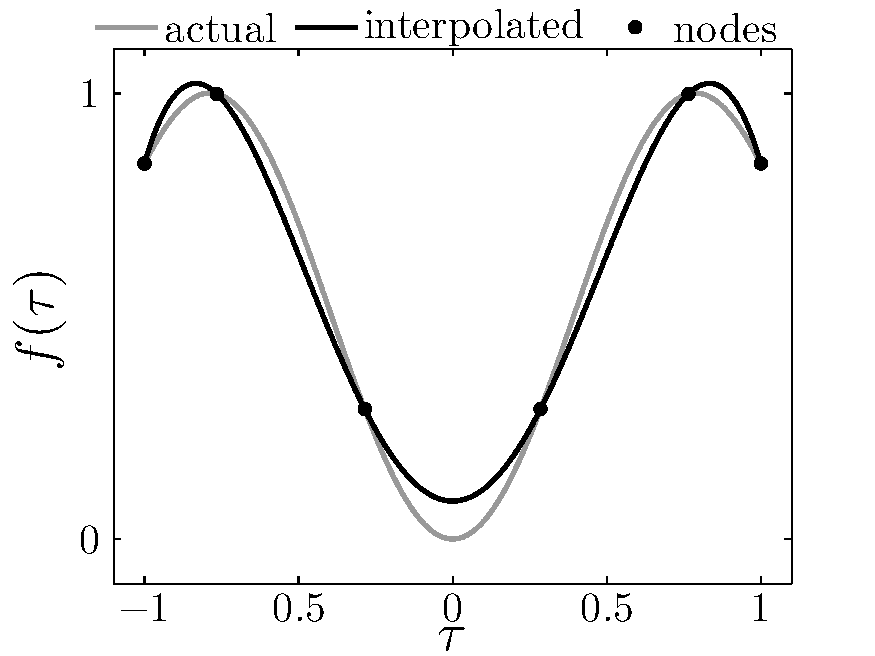
\includegraphics[width=0.33\textwidth, trim=0in 0in 0.5in 0in,clip=true]{../app3/figures/diff-1}%
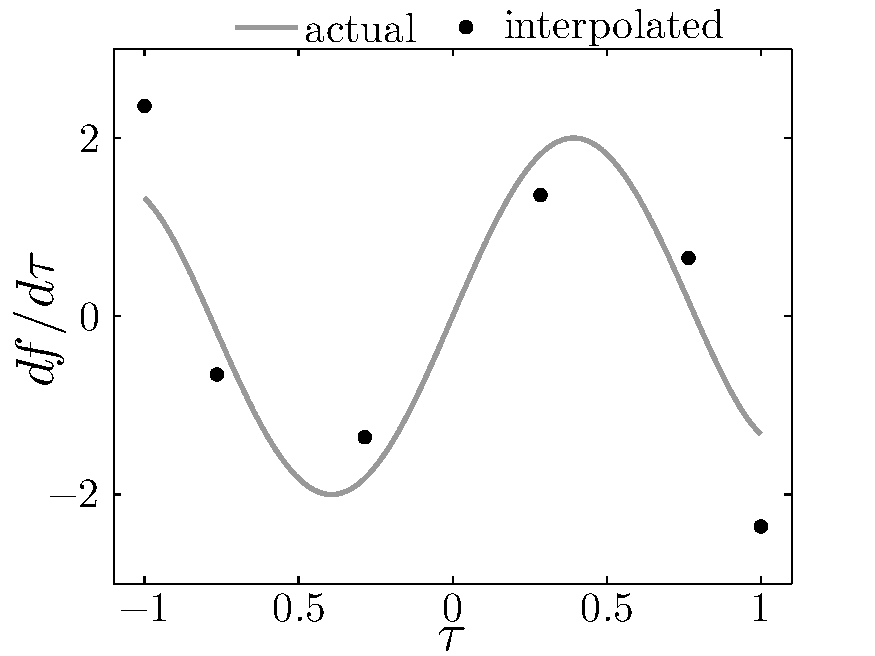
\includegraphics[width=0.33\textwidth, trim=0in 0in 0.5in 0in,clip=true]{../app3/figures/diff-2}%
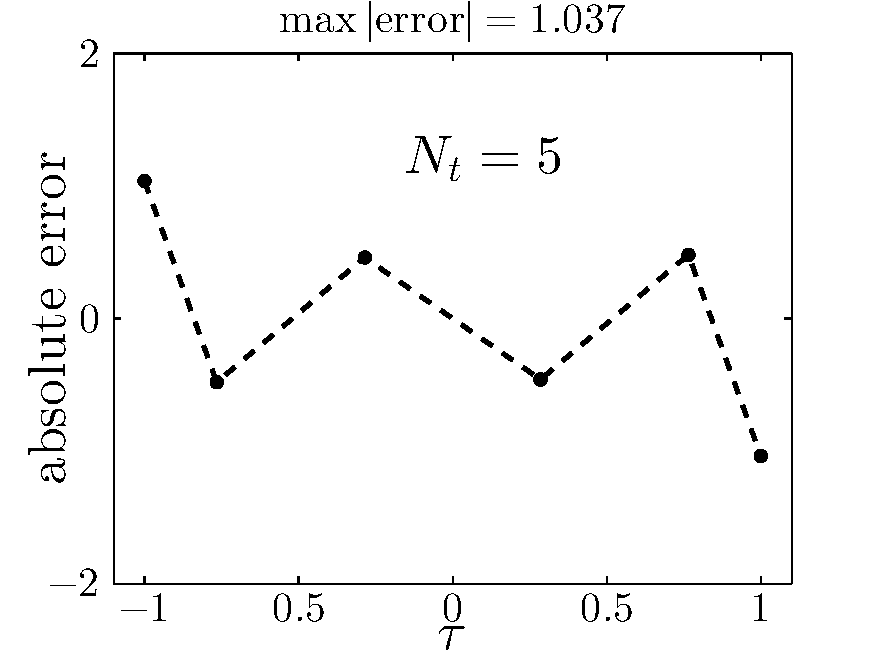
\includegraphics[width=0.33\textwidth, trim=0in 0in 0.5in 0in,clip=true]{../app3/figures/diff-3}%

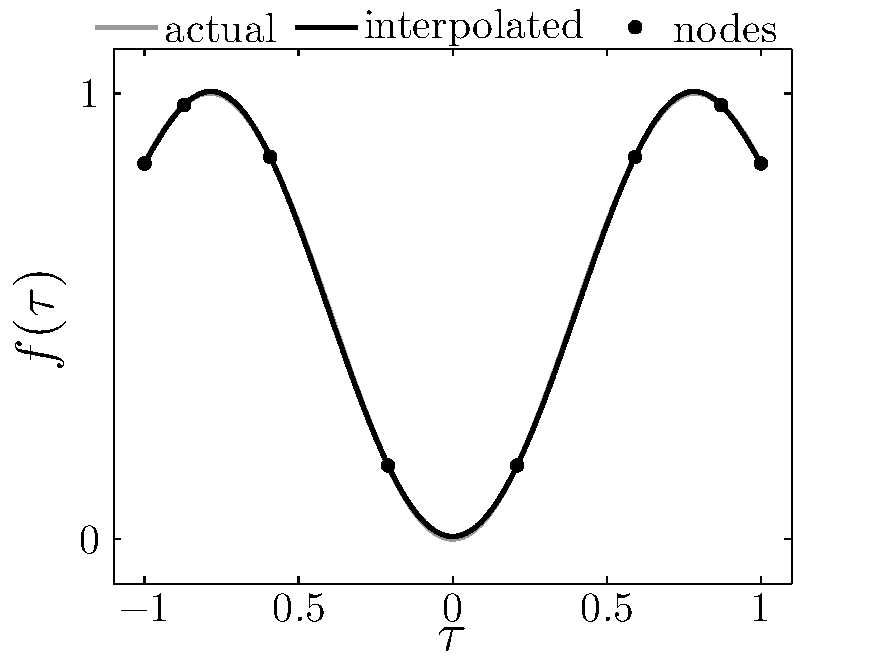
\includegraphics[width=0.33\textwidth, trim=0in 0in 0.5in 0in,clip=true]{../app3/figures/diff-4}%
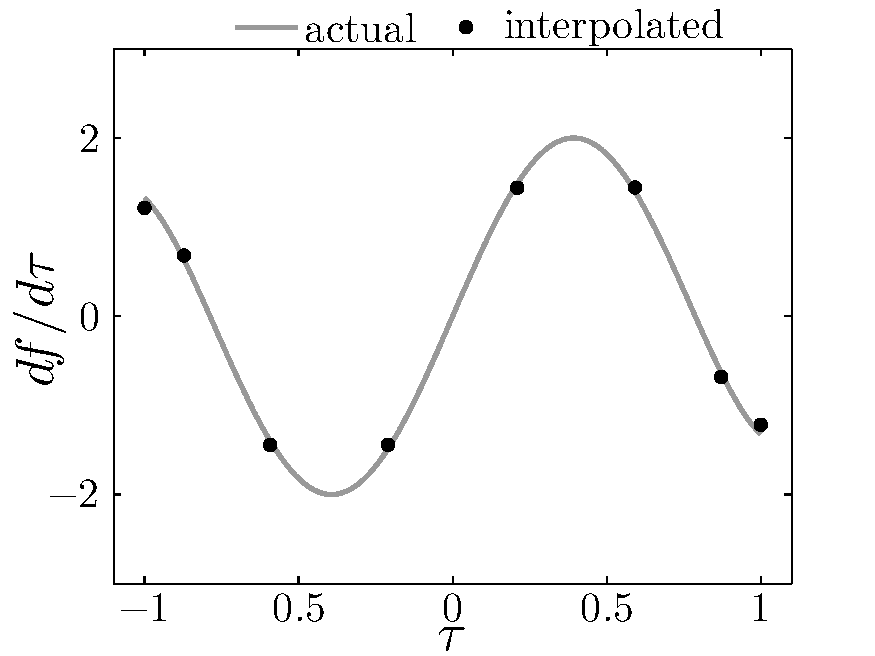
\includegraphics[width=0.33\textwidth, trim=0in 0in 0.5in 0in,clip=true]{../app3/figures/diff-5}%
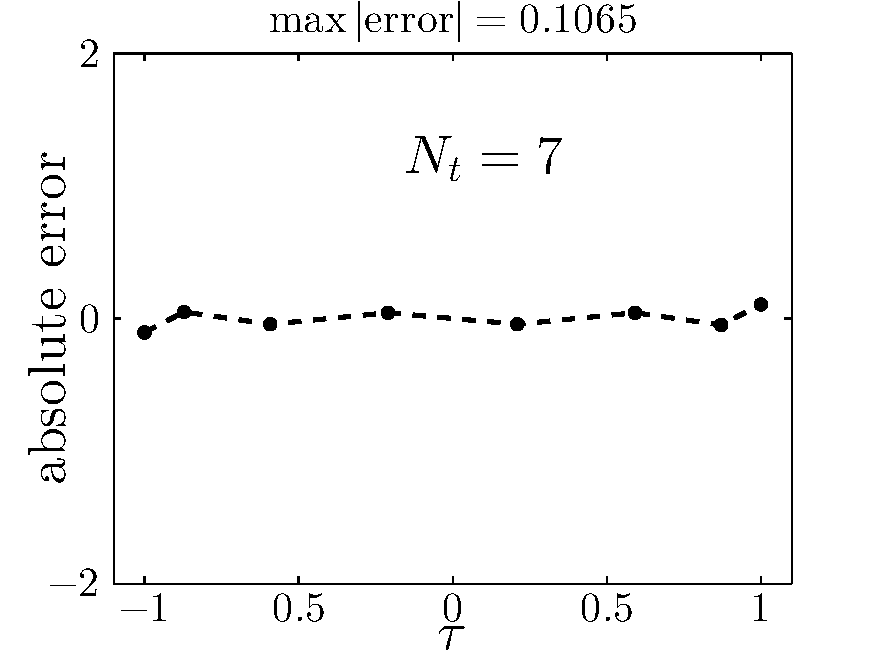
\includegraphics[width=0.33\textwidth, trim=0in 0in 0.5in 0in,clip=true]{../app3/figures/diff-6}%

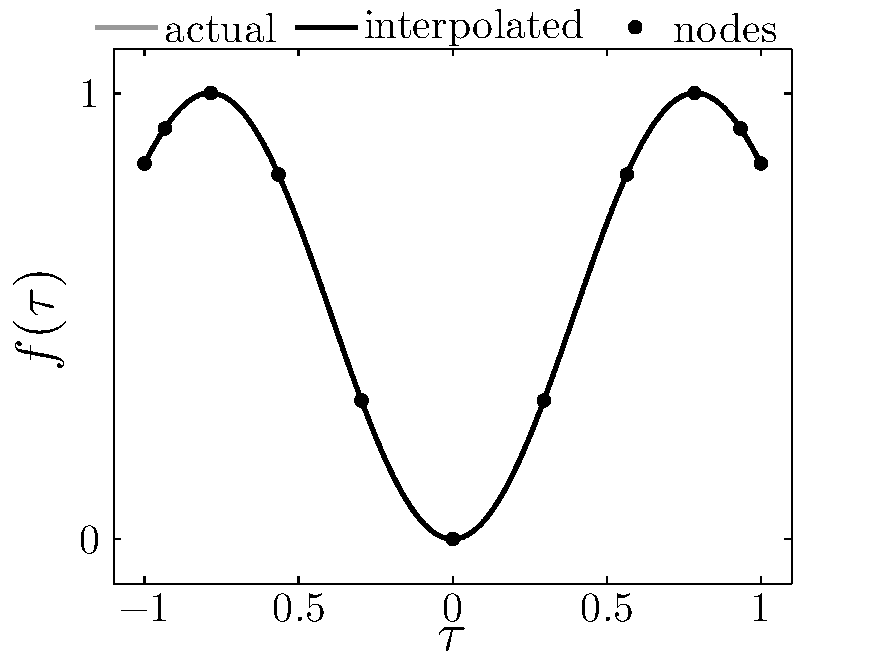
\includegraphics[width=0.33\textwidth, trim=0in 0in 0.5in 0in,clip=true]{../app3/figures/diff-7}%
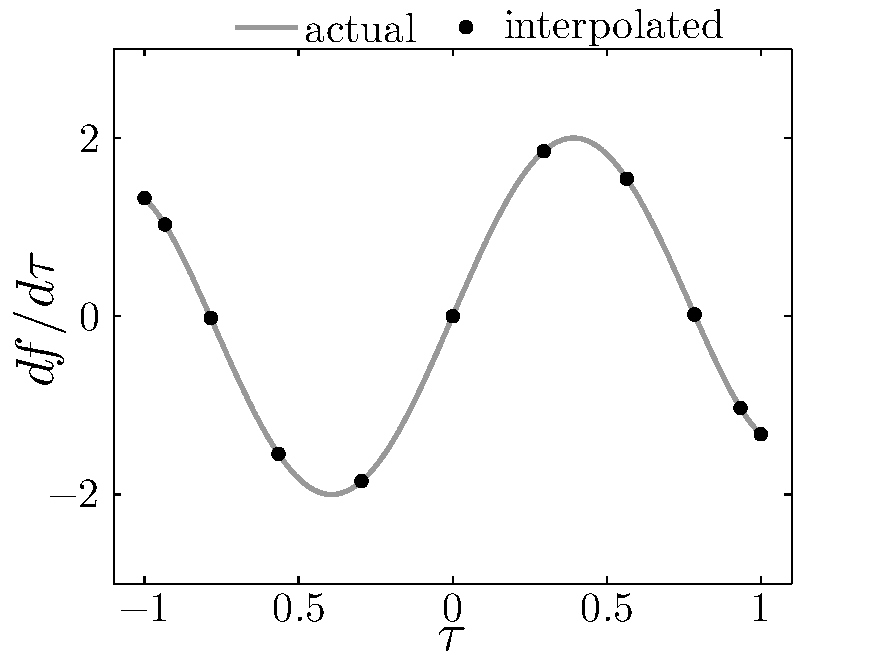
\includegraphics[width=0.33\textwidth, trim=0in 0in 0.5in 0in,clip=true]{../app3/figures/diff-8}%
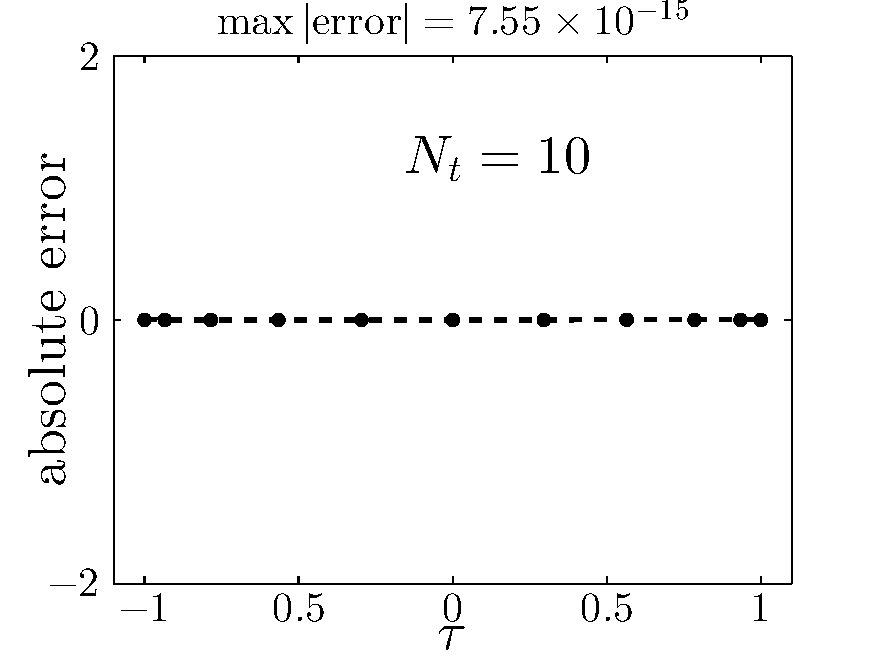
\includegraphics[width=0.33\textwidth, trim=0in 0in 0.5in 0in,clip=true]{../app3/figures/diff-9}%

\caption[Differentiation error using Lagrange interpolation with LGL nodes]{Differentiation error using Lagrange interpolation with LGL nodes for various values of $N_t$.\label{fig:diff}}

\end{figure}